The default Flowers 102 split is already low-data (ten images per class). We test how each method behaves as the training budget shrinks further, which is the setting where parameter-efficient tuning should help most.

\subsection{Experimental Setup}
For $k \in \{1, 2, 5\}$, we subsample the training set to $k$ images per class (first $k$ per class, deterministic with seed 69). The validation and test sets are unchanged. We train for 30 epochs (shorter because the dataset is smaller) with the same optimizer and schedule as the full-data experiments. We use the same six methods for every $k$.

\subsection{Results and Analysis}
Figure~\ref{fig:fewshot} plots the best validation accuracy at each $k$.

\begin{figure}[H]
\centering
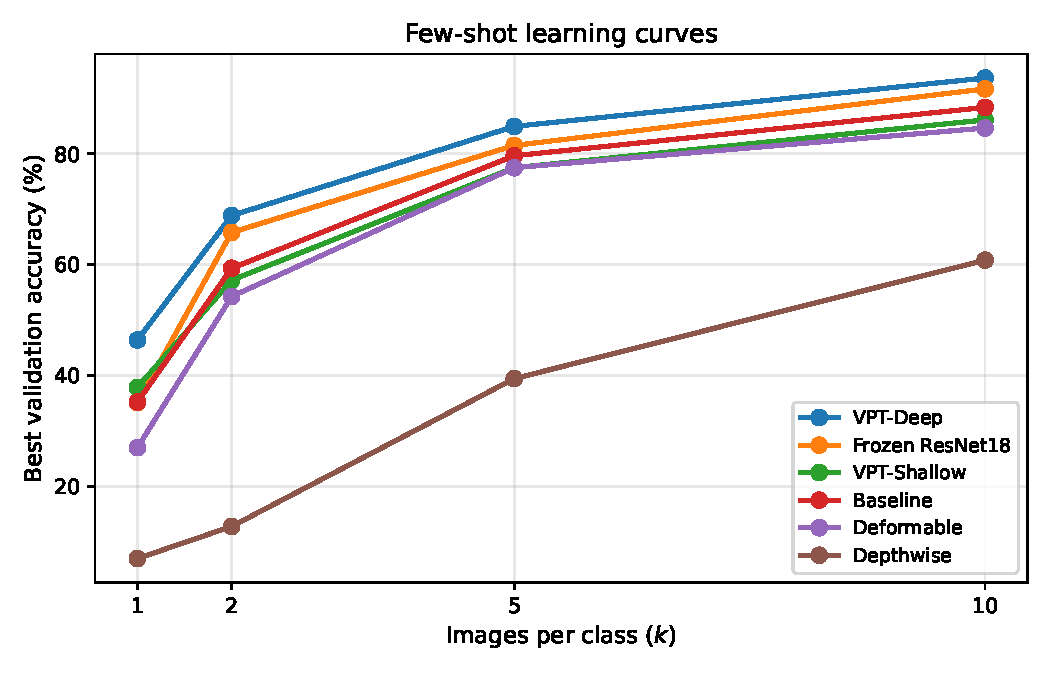
\includegraphics[width=0.75\textwidth]{figures/fewshot-curves.pdf}
\caption{Few-shot learning curves. VPT-Deep dominates across all $k$.}
\label{fig:fewshot}
\end{figure}

\begin{table}[H]
\centering
\small
\begin{tabular}{lcccc}
\toprule
Method & $k{=}1$ & $k{=}2$ & $k{=}5$ & $k{=}10$ \\
\midrule
VPT-Deep           & \textbf{46.37} & \textbf{68.82} & \textbf{84.90} & \textbf{93.63} \\
Frozen ResNet18    & 35.10 & 65.78 & 81.47 & 91.67 \\
VPT-Shallow        & 37.84 & 57.16 & 77.45 & 86.08 \\
Baseline (full FT) & 35.20 & 59.31 & 79.61 & 88.33 \\
Deformable         & 26.96 & 54.22 & 77.45 & 84.61 \\
Depthwise          & 6.96  & 12.75 & 39.41 & 60.78 \\
\bottomrule
\end{tabular}
\caption{Best validation accuracy (\%) at different training budgets.}
\label{tab:fewshot}
\end{table}

VPT-Deep wins at every $k$. The margin over the frozen ResNet18 is roughly one point at $k=10$, three points at $k=5$, three points at $k=2$, and eleven points at $k=1$. Low-data regimes widen the gap, which matches the central message of \citet{jia2022vpt}: with fewer labelled examples, updating fewer parameters is the right move. The baseline (which fine-tunes 11M parameters) sits below both VPT and the frozen ResNet18 at small $k$, and catches up only at $k=10$.

Depthwise-separable collapses at low $k$ (6.96\% at $k=1$) because it starts from randomly initialised weights and cannot recover with so few examples. Deformable convolution is also hurt at small $k$: the offset predictor needs more data to learn useful displacements than is available.

Put together with Table~\ref{tab:main-results}, the few-shot curves are the strongest version of our thesis: the less data you have, the more you should lean on pre-trained features, and the less you should modify the backbone.
